\section{Auswertung}

Die Abb.  \ref{fig:00mm} und \ref{fig:10mm} zeigen die von der Kamera aufgenommenen Bilder beispielhaft für die Extrempositionen der gemessenen Verschiebung. Da die Reflexion eines Lasers nicht in einem Punkt lokalisiert ist, wurde die genaue Position der Abbildung auf dem Kamerasensor vergleichend mittels zwei verschiedener Verfahren ermittelt.

Für beide Verfahren wurde zunächst die Intensität spaltenweise aufsummiert.

Die einfachere Variante ermittelte nun die Position $px_m$ auf dem CCD-Sensor in Pixeln  durch Auswahl der Spalte mit der größten Intensitätssumme als Zentrum des Laserpunkts. Die Genauigkeit dieses Verfahrens ist folglich gleich oder kleiner der Sensorauflösung, die Pixelangabe somit ganzzahlig.

Alternativ wurde die Position subpixelgenau über eine Regression ermittelt. Hierfür wurde die Intensitätsverteilung des Lasers als gaußförmig angenommen. In der logarithmiertem Darstellung entspricht das einer Parabel, für welche eine Regression leicht durchgeführt werden kann. Der Scheitelpunkt dieser Parabel wurde als Position $px_g$ in Pixeln verwendet. Dieses Verfahren kann die Position mit einer Genauigkeit über der Pixelauflösung bestimmen.

Die so bestimmte Pixelposition entspricht (nach Differenzbildung mit einem Referenzpunkt, in diesem Fall $z=0$) gemäß Gl. (\ref{eq:zfinal}) einer $z$-Verschiebung $z_m$ bzw. $z_g$.

In Tab. \ref{tab:messwerte} sind die ermittelten Größen ersichtlich.

Zum Vergleich der beiden Verfahren wurden aus ermittelter und bekannter (da eingestellter) Verschiebung die absoluten $\Delta z_{m,g}$ und relativen Fehler $|\Delta z_{m,g}/z|$ für jedes der Wertetupel errechnet. Man erkennt schnell, dass das Regressionsverfahren nicht nur subpixelgenau ist, sondern auch viel geringere stochastische Fehler macht. Es zeigt bezüglich der Intensitätsverteilung Tiefpassverhalten. Der in Abb. \ref{fig:plot_rel} ersichtliche Verlauf des Fehlers ist vorhersehbar und kann folglich bei bekanntem Messaufbau herausgerechnet werden, was die Genauigkeit noch weiter steigert.

Zusammenfassend ist das Gaußkurven-Regressionsverfahren somit besser geeignet, wenn Ortsbestimmung sehr genau erfolgen muss. Es erfordert jedoch auch eine deutlich höhere Rechenleistung. Daher hat das Maximalwertsverfahren die bessere Echtzeitfähigkeit.

\begin{figure}[tbh]
	\centering
	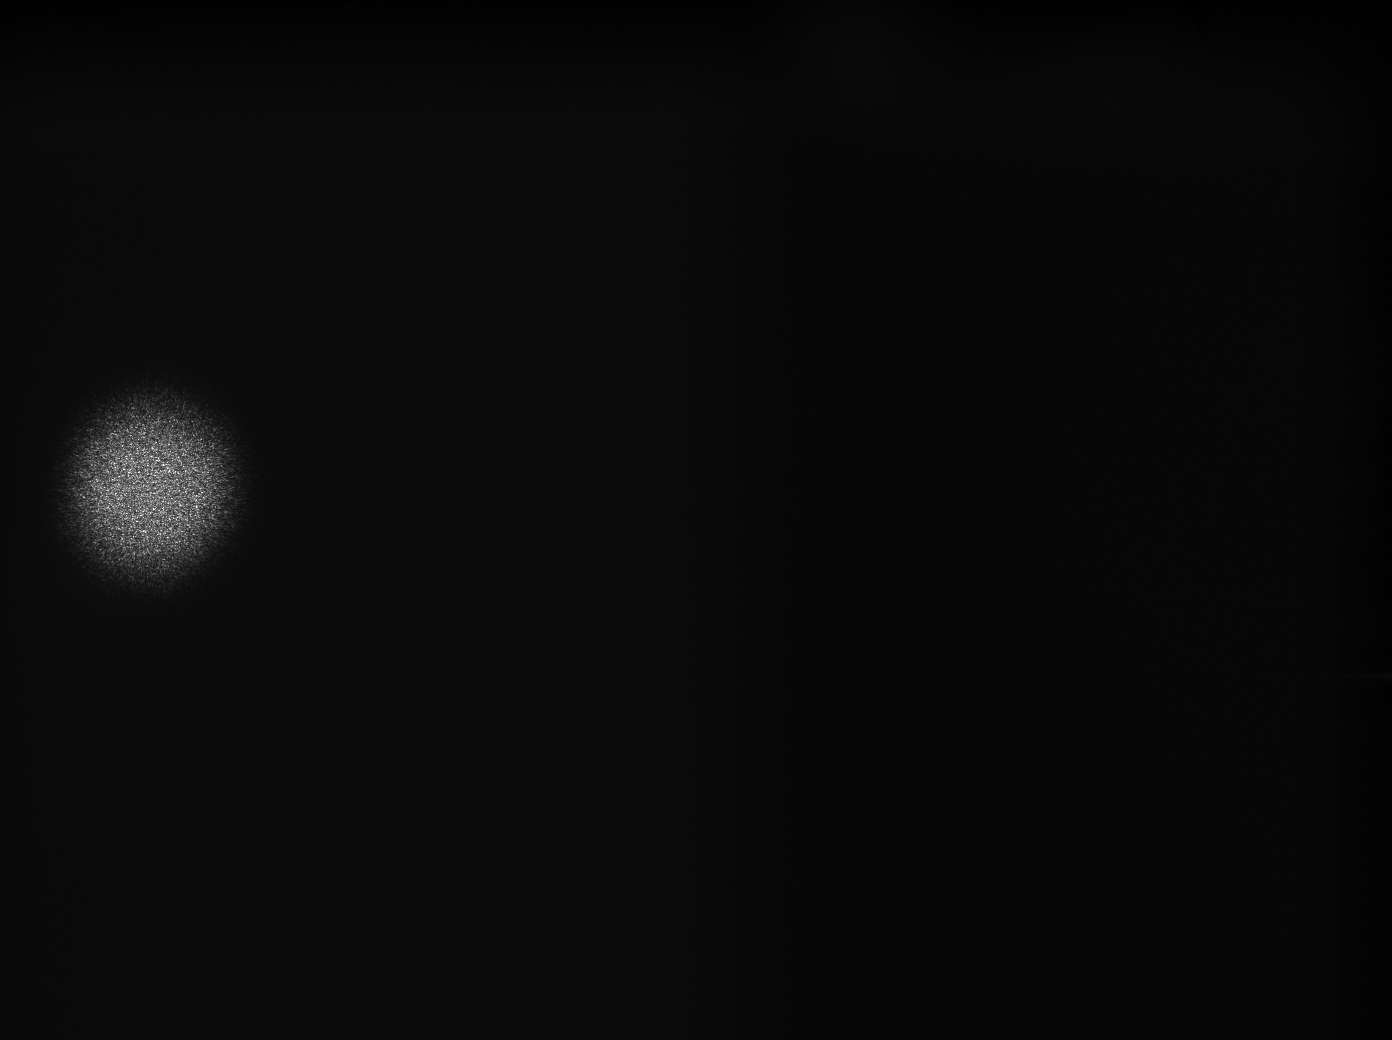
\includegraphics[width=0.8\linewidth]{img/00cm.jpg}
	\caption{Aufnahme für $z=0$}
	\label{fig:00mm}
\end{figure}

\begin{figure}[tbh]
	\centering
	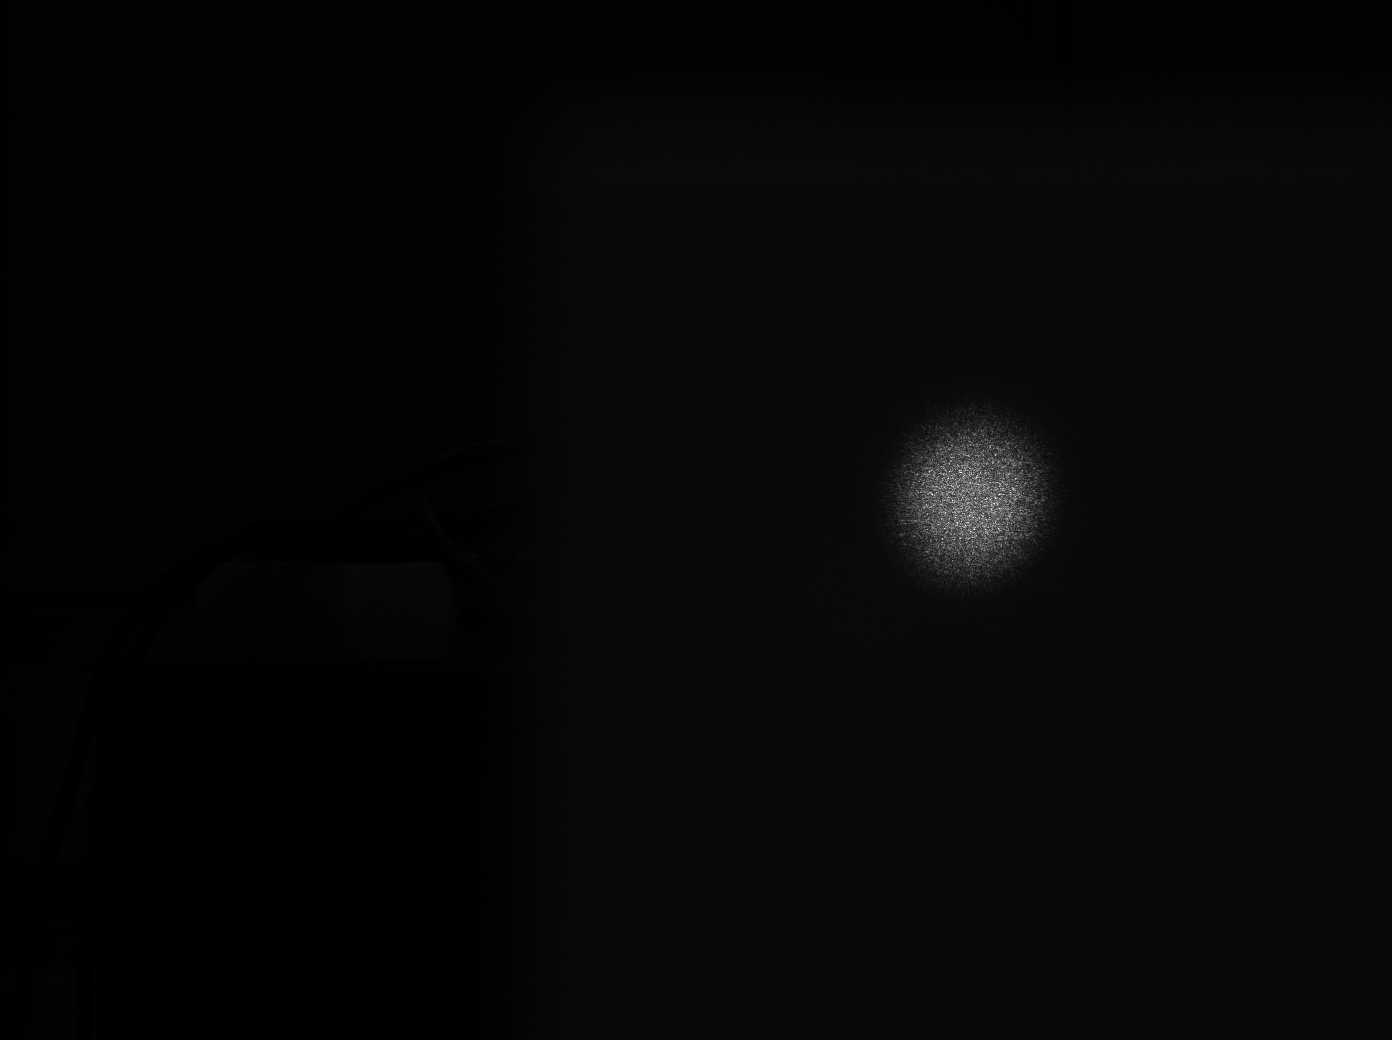
\includegraphics[width=0.8\linewidth]{img/100cm.jpg}
	\caption{Aufnahme für $z=\SI{10}{\mm}$}
	\label{fig:10mm}
\end{figure}

\begin{table}[tbh]
	\centering
	\pgfplotstabletypeset[
	col sep=comma,
	precision = 2,
	fixed,
	dec sep align,
	every head row/.style={,after row=\hline},
	every last row/.style={after row=\hline},
	columns={d,png,pnm,dg,dm,afg,afm,rfg,rfm},
	columns/d/.style={column name=$z/\si{\milli\meter}$},
	columns/png/.style={column name=$px_g$},
	columns/pnm/.style={column name=$px_m$},
	columns/dg/.style={column name=$z_g/\si{\milli\meter}$},
	columns/dm/.style={column name=$z_m/\si{\milli\meter}$},
	columns/afg/.style={column name=$\Delta z_g/\si{\milli\meter}$},
	columns/afm/.style={column name=$\Delta z_m/\si{\milli\meter}$},
	columns/rfg/.style={column name=$|\Delta z_g/z|/\%$},
	columns/rfm/.style={column name=$|\Delta z_m/z|/\%$},	
	]{./tab/Triangulation.csv}
	\caption{Messwerte}
	\label{tab:messwerte}
\end{table}

\begin{figure}[tbh]
	\centering
	\begin{tikzpicture}[trim axis left, trim axis right]
	\begin{axis}[width=0.9\textwidth,
	height=0.35\textheight,
	%y label style = {rotate=-90},
	%y tick label style={/pgf/number format/.cd,fixed, fixed zerofill},
	%x tick label style={/pgf/number format/.cd,fixed, fixed zerofill},
	grid=both,                     
	%title={Der Titel}, 
	xlabel={$z/\si{\milli\meter}$}, 
	ylabel={Absolute Fehler in $\si{\milli\meter}$},
	ybar,
	bar width = 7pt,
	xmin=-5,
	xmax=105,
	%ymin=0,
	%ymax=4,
	%xtick={0,0.2,0.4,0.6,0.8,1},
	legend pos = south east,
	legend cell align = left,
	legend entries={$|\Delta z_g|$, $|\Delta z_m|$}
	]                
	%\addlegendimage{mark=*, color=red}
	%\addlegendimage{mark=*, color=blue}     
	\addplot[blue, fill] table[x=d, y=afg, col sep=comma]{./tab/Triangulation.csv};
	\addplot[red, fill] table[x=d, y=afm, col sep=comma]{./tab/Triangulation.csv};
	\end{axis}
	\end{tikzpicture}
	\caption{Absolute Fehler}
	\label{fig:plot_abs}
\end{figure}

\begin{figure}[tbh]
	\centering
	\begin{tikzpicture}[trim axis left, trim axis right]
	\begin{axis}[width=0.9\textwidth,
	height=0.35\textheight,
	%y label style = {rotate=-90},
	%y tick label style={/pgf/number format/.cd,fixed, fixed zerofill},
	%x tick label style={/pgf/number format/.cd,fixed, fixed zerofill},
	grid=both,                     
	%title={Der Titel}, 
	xlabel={$z/\si{\milli\meter}$}, 
	ylabel={Relativer Fehler in $\%$},
	ybar,
	bar width = 7pt,
	xmin=-5,
	xmax=105,
	ymin=0,
	%ymax=4,
	%xtick={0,0.2,0.4,0.6,0.8,1},
	legend pos = north east,
	legend cell align = left,
	legend entries={$\Delta z_g/z$, $\Delta z_m/z$}
	]                
	%\addlegendimage{mark=*, color=red}
	%\addlegendimage{mark=*, color=blue}     
	\addplot[yellow!90!black, fill] table[x=d, y=rfg, col sep=comma]{./tab/Triangulation.csv};
	\addplot[green!60!black, fill] table[x=d, y=rfm, col sep=comma]{./tab/Triangulation.csv};
	\end{axis}
	\end{tikzpicture}
	\caption{Relative Fehler}
	\label{fig:plot_rel}
\end{figure}